\documentclass{article}
%% Preemptively pass options to avoid import conflicts.
\PassOptionsToPackage{linesnumbered,ruled,vlined}{algorithm2e}
\PassOptionsToPackage{english}{babel}
\PassOptionsToPackage{capitalise,noabbrev}{cleveref}
\PassOptionsToPackage{pdftex}{graphicx}
\PassOptionsToPackage{bookmarks}{hyperref}
\PassOptionsToPackage{utf8}{inputenc}
\PassOptionsToPackage{newfloat}{minted}
\PassOptionsToPackage{numbers,compress}{natbib}
\PassOptionsToPackage{dvipsnames}{xcolor}

\usepackage{adjustbox}
\usepackage{algorithm2e}
\usepackage{amsfonts}
\usepackage{amsmath}
\usepackage{amssymb}
\usepackage{babel}
\usepackage{bm}
\usepackage{booktabs}
\usepackage{cancel}
\usepackage{caption}
\usepackage{enumitem}
\usepackage{etoolbox}
\usepackage{fancyvrb}
\usepackage{graphicx}
\usepackage{inputenc}
\usepackage{kantlipsum}
\usepackage{listings}
\usepackage{mathtools}
\usepackage{minted}
\usepackage{natbib}
\usepackage{nicefrac}
\usepackage{svg}
\usepackage{tikz}
\usepackage{verbatim}
\usepackage{wrapfig}
\usepackage{xcolor}

%% Load these after everything else.
\usepackage{hyperref}
\usepackage{cleveref}

%% Skip spacing around equation display (use inside document environment).
\newcommand{\displayskip}[1]{
  \setlength{\abovedisplayskip}{#1}
  \setlength{\belowdisplayskip}{#1}
  \setlength{\abovedisplayshortskip}{#1}
  \setlength{\belowdisplayshortskip}{#1}
}

%% TikZ settings
\usetikzlibrary{positioning,arrows.meta,quotes,shapes,bayesnet}
\tikzset{>=latex}

%% Cleveref settings
\crefname{equation}{}{}
\Crefname{equation}{}{}

%%
% Conference specific toggles when needed.
% Usage: \iftoggle{name}{true}{false}
%
\newtoggle{icml} \togglefalse{icml}
\newtoggle{neurips} \togglefalse{neurips}
\newtoggle{aistats} \togglefalse{aistats}

%% Text highlights.
\newcommand{\info}[1]{\textcolor{ForestGreen}{\textbf{#1}}}
\newcommand{\warn}[1]{\textcolor{RedOrange}{\textbf{#1}}}

%% natbib settings
\renewcommand{\bibname}{References}
\bibliographystyle{plainnat}

%% Wrapping minted code listings
\newenvironment{code}{\captionsetup{type=listing}}{}

%% Symbols
\newcommand{\gp}{\ensuremath{\mathcal{GP}}}  % GP
\newcommand{\kl}{\ensuremath{\mathcal{KL}}}  % KL-divergence
\newcommand{\gaussian}[1]{\ensuremath{\mathcal{N}\left(#1\right)}}  % Gaussian
\newcommand{\defeq}{\ensuremath{\triangleq}}  % definition

% \DeclarePairedDelimiter{\ceil}{\lceil}{\rceil}
% \DeclarePairedDelimiter{\floor}{\lfloor}{\rfloor}
\newcommand{\ceil}[1]{\ensuremath{\left\lceil #1 \right\rceil}}
\newcommand{\floor}[1]{\ensuremath{\left\lfloor #1 \right\rfloor}}

\newcommand{\determ}[1]{\ensuremath{\left\lvert#1\right\rvert}}  % determinant
\newcommand{\logdet}[1]{\ensuremath{\log{\determ{#1}}}}
\newcommand{\norm}[1]{\ensuremath{\left\lVert#1\right\rVert}}  % norm
\newcommand{\ci}{\ensuremath{\mathrel{\perp\mspace{-10mu}\perp}}}  % conditional independence
\newcommand{\nci}{\ensuremath{\cancel{\ci}}}  % conditional dependence

\newcommand{\tr}[1]{\text{tr}\ensuremath{\left(#1\right)}}
\newcommand{\pd}[2]{\ensuremath{\frac{\partial #1}{\partial #2}}}

%% Transforms
\newcommand{\mbf}[1]{{\ensuremath{\boldsymbol{\mathbf{#1}}}}}  % bold math
\newcommand{\vrb}[1]{\Verb+#1+}  % verbatim

%% Variables
\newcommand{\reals}{\ensuremath{\mathbb{R}}}  % real numbers
\newcommand{\naturals}{\ensuremath{\mathbb{N}}}  % natural numbers
\newcommand{\ints}{\ensuremath{\mathbb{Z}}}  % integers
\newcommand{\dset}{\ensuremath{\mathcal{D}}}  % Dataset
\newcommand{\xvec}{\mbf{x}}  % vector x
\newcommand{\yvec}{\mbf{y}}  % vector y
\newcommand{\Xvec}{\mbf{X}}  % vector X (caps)
\newcommand{\Yvec}{\mbf{Y}}  % vector Y (caps)
\usepackage[margin=1in]{geometry}

\setlength{\parindent}{0em}
\setlength{\parskip}{1em}

\title{Example \LaTeX{ }file}
\author{Sanyam Kapoor}

\begin{document}

\maketitle

\section{Symbols}

\begin{enumerate}%[label=(\alph*)]
\item Reals \vrb{\reals}: \reals
\item Naturals \vrb{\naturals}: \naturals
\item Integers \vrb{\ints}: \ints
\item Bold symbols \vrb{\mbf{}}: \mbf{\Sigma}, \mbf{X}, $\dots$
\item Definition \vrb{\defeq}: \defeq
\item Determinant \vrb{\determ{}}: \determ{\cdot}
\item logdet \vrb{\logdet{}}: \logdet{\cdot}
\item Norm \vrb{\norm{}}: \norm{\cdot}
\item Conditional independence \vrb{\ci},\vrb{\nci}: \ci, \nci
\item Gaussian Process \vrb{\gp}: \gp
\item KL-divergence \vrb{\kl}: \kl
\item Gaussian distribution \vrb{\gaussian{}}: \gaussian{\cdot, \cdot}
\item Trace \vrb{\tr{}}: \tr{\cdot}
\item Partial derivative \vrb{\pd{}{}}: \pd{f}{x}(x)
\item Ceiling \vrb{\ceil{\frac{n}{k}}}: $\ceil{\frac{n}{k}}$
\item Floor \vrb{\floor{\frac{n}{k}}}: $\floor{\frac{n}{k}}$
\end{enumerate}

\section{Code Snippets}

\begin{code}
\caption{Source code example} \label{code:sample}
\inputminted[firstline=1,lastline=2,fontsize=\small]{python}{test.py}
\end{code}

\section{Media}

\vrb{\includesvg{}} may or may not work. Alternatively, convert to PDF which works reliably with Altair charts. See \cref{fig:svg_pdf}.

% \begin{wrapfigure}{r}{0.6\textwidth}
\begin{figure}[ht]
    \centering
    \begin{tabular}{ccc}
        \includesvg[width=0.15\linewidth]{favicon} & 
\includegraphics[width=0.15\linewidth]{favicon.pdf} &
        \includesvg[width=0.3\linewidth]{bayes} \\
        (a) & (b) & (c)
    \end{tabular}
    \caption{SVG loaded from a (a) \texttt{.svg} file, and as a (b) \texttt{.pdf} file. (c) \emph{The Church of Bayes}. }
    \label{fig:svg_pdf}
\end{figure}    
% \end{wrapfigure}

\subsection{Placeholders}

A placeholder is provided in \cref{fig:svg_pdf}(c) for the waiting times until the graphs/plots are ready.

\subsubsection{Example Images}

\begin{figure}[!ht]
\centering
\begin{tabular}{cc}
    \includegraphics[width=0.49\linewidth]{example-image-a} & \includegraphics[width=0.49\linewidth]{example-image-b} \\
    (a)\vrb{\includegraphics{example-image-a}} & (b) \vrb{\includegraphics{example-image-a}}
\end{tabular}
\caption{Example images from built-in package.}
\label{fig:my_label}
\end{figure}

\section{Equations, Citations, Figures}

References work with \vrb{\citet{vargp2020}}, rendered as \citet{vargp2020}.

\begin{align}
p(\theta \mid \xvec) = \frac{p(\xvec\mid\theta)p(\theta)}{p(\xvec)} \label{eq:bayesrule}
\end{align}

Some clever reference examples using \texttt{Cleveref} package.

\begin{enumerate}
\item Equations \vrb{\cref{eq:bayesrule}}: \cref{eq:bayesrule}.
\item Figures \vrb{\cref{fig:svg_pdf}}: \cref{fig:svg_pdf}.
\item Code \vrb{\cref{code:sample}}: \cref{code:sample}.
\end{enumerate}

\section{Dummy text}

Use \vrb{\kant[1-3]} to get multiple paragraphs. Or, just a single digit to get the specific pseudokantian paragraph.

\kant[1-3]

\section{Simple Bayesian Network}

See \cref{fig:bayes_net} for an example of a simple \emph{Bayesian network} for linear regression.

\begin{figure}[ht]
    \centering
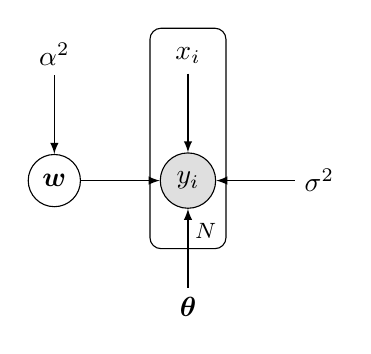
\begin{tikzpicture}
    \node [obs] (y) at (0,0) {$y_i$};
    \node [mark size=2pt,color=black,above=of y] (X) {$x_i$};
    \node [mark size=2pt,color=black,below=of y] (theta) {$\mbf{\theta}$};
    \node[circle,draw=black,fill=white,left=of y] (w) {$\bm{w}$};
    \node [mark size=2pt,color=black,above=of w] (alpha) {$\alpha^2$};
    \node [mark size=2pt,color=black,right=of y] (var) {$\sigma^2$};
    
    \path [draw,->] (theta) edge (y);
    \path [draw,->] (X) edge (y);
    \path [draw,->] (w) edge (y);
    \path [draw,->] (var) edge (y);
    \path [draw,->] (alpha) edge (w);

    \plate [color=black] {obs_plate} {(X)(y)} {$N$};
\end{tikzpicture}
    \caption{A simple Bayesian network for linear regression.}
    \label{fig:bayes_net}
\end{figure}

% \bibliographystyle{plainnat}
\bibliography{refs}

\end{document}